\documentclass[12pt]{article}

\usepackage[margin=1in]{geometry}
\usepackage{amsmath,amsthm,amssymb}
\usepackage{tikz} % for drawing stuff
\usepackage{xcolor} % for \textcolor{}
\usepackage{readarray} % for \getargsC{}
\usepackage{graphicx} % disjoint union
\usepackage[utf8]{inputenc}
\usepackage[T1]{fontenc}
\usepackage{hyperref}


% Math sets
\newcommand{\N}{\mathbb{N}}
\newcommand{\Z}{\mathbb{Z}}
\newcommand{\R}{\mathbb{R}}

% Setup of project
\newenvironment{question}[2][Question]{\begin{trivlist}
\item[\hskip \labelsep {\bfseries #1}\hskip \labelsep {\bfseries #2.}]}{\end{trivlist}}
\newenvironment{answer}[2][Answer]{\begin{trivlist}
\item[\hskip \labelsep {\bfseries #1}\hskip \labelsep {\bfseries #2:}]}{\end{trivlist}}
\begin{document}
% math enumerate
\renewcommand{\theenumi}{\roman{enumi}}

% Short hands
\let\oldsum\sum
\renewcommand{\sum}[3]{\oldsum\limits_{#1}^{#2}#3}
\let\oldprod\prod
\renewcommand{\prod}[3]{\oldprod\limits_{#1}^{#2}#3}


\title{Homework 3}
\author{Haukur Páll Jónsson\\
NLP 2017}

\maketitle

\begin{question}{1}
CCG parsing
\end{question}
\begin{answer}{a)}{}

Each rule application is given with \\
|word part 1 + word part 2| resulting category | rule applied

The ordering of rule application is:\\
1. |two + units| N | Forward appliaction \\
2. |the + two units| NP | Forward appliaction \\
3. |to + the two units| PP | Forward appliaction \\
4. |four + Boeign-747s| NP | Forward appliaction \\
5. |The + company| NP | Forward appliaction \\
6. |added + four Boeign-747s| (S $\backslash\backslash$ NP)/PP | Forward appliaction \\
7. |added four Boeign-747s + to the two units| S $\backslash\backslash$ NP | Forward appliaction \\
8. |in + 1994| (S  NP)$\backslash\backslash$(S $\backslash\backslash$ NP) | Forward appliaction \\
9. |added four Boeign-747s to the two units + in 1994| (S $\backslash\backslash$ NP) | Backward appliaction \\
10. |The company + added four Boeign-747s to the two units in 1994| S | Backward appliaction \\
\end{answer}

\begin{question}{2}
Max-ent models
\end{question}

\begin{answer}{a)}

A maximum entropy model predicts the most likely $y$ given $\boldsymbol{x}$. For each y we compute:
$$P(y|\boldsymbol{x})=\frac{e^{w \cdot f(\boldsymbol{x},y)}}{Z}$$
Where $Z=\sum{y'}{}{w \cdot f(\boldsymbol{x}, y')}$ is a normalizing constant.
We can take the log of this expression and still get the same prediction as the logarithm is monotonically increasing:
$$\log{P(y|\boldsymbol{x})}=\frac{w \cdot f(\boldsymbol{x},y)}{\log{Z}}$$
$$\log{P(y|\boldsymbol{x})}=\sum{i=1}{k}{w_i * f_i(\boldsymbol{x},y)} - \log{Z}$$
The maximum entropy model is called a log linear model since if you take the logarithm of the expression, the model is simply a linear combination of its parameters.
\end{answer}
\begin{answer}{b)}

Now we compute $\sum{i=1}{k}{w_i * f_i(\boldsymbol{x},y)}$ for each y. Note that $animal$ does not appear in the text ($\boldsymbol{x}$) so $f_4$ to $f_6$ are always zero.

$$\sum{i=1}{9}{w_i * f_i(\boldsymbol{x},1)}=2-0.1=1.9$$
$$\sum{i=1}{9}{w_i * f_i(\boldsymbol{x},2)}=1.8+1.1=2.9$$
$$\sum{i=1}{9}{w_i * f_i(\boldsymbol{x},1)}=0.3+2.7=3.0$$
$$Z=\log{(e^{1.9}+e^{2.9}+e^3)}=3.8054$$
Thus,
$$P(y=1|\boldsymbol{x})=1.9-3.8054=-1.9054$$
$$P(y=2|\boldsymbol{x})=2.9-3.8054=-0.9054$$
$$P(y=3|\boldsymbol{x})=3.0-3.8054=-0.8054$$
We can verify that this is indeed correct: $e^{-1.9054} + e^{-0.9054} + e^{-0.8054} = 1.0$. The most probable sense is $y=3$, a noun.
\end{answer}

\begin{question}{3}
First order logic to natural language
\end{question}

\begin{answer}{a)}{}

All bears are furry
\end{answer}
\begin{answer}{b)}{}

Sergii is eating a pizza with a fork
\end{answer}
\begin{answer}{c)}{}

(All) the students lift Marie
\end{answer}
\begin{answer}{d)}{}

The students lifted Marie
\end{answer}

\begin{question}{4}
Natural language to first order logic
\end{question}

\begin{answer}{a)}{Juan hates pasta}

$$\exists\, e,x \, hating(e) \land hater(e, Juan) \land hated(e, x) \land pasta(x) $$
\end{answer}
\begin{answer}{b)}{Some student likes every class}

This sentence is ambigious, it can mean "A single student likes each and every class" or "Each student likes some class but possibly different classes". The first sentence:

$$\exists \, s. \, student(s) \land \forall \, c. \, class(c) \implies likes(s,c)$$
And the other sentence:
$$\forall \, s. \, student(s) \implies \exists \, c. \, class(c) \land likes(s,c)$$
\end{answer}

\begin{question}{5}
Semantic attachments
\end{question}
\begin{answer}{a)}{}

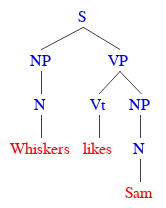
\includegraphics[scale=0.5]{sem_parse_grapg}
The parse for the sentence is given by the figure. Then we compute the semantics of the sentence:
\begin{align*}
S.sem &=VP.sem(NP.sem) \\
&=VP.sem(N.sem) \\
&=VP.sem(Whiskers) \\
&=Vt.sem(NP.sem)(Whiskers) \\
&=Vt.sem(N.sem)(Whiskers) \\
&=Vt.sem(Sam)(Whiskers) \\
&=\lambda x.\lambda y. \exists e. liking(e) \land liker(e,y) \land likee(e,x)(Sam)(Whiskers) \\
&=\lambda y. \exists e. liking(e) \land liker(e,y) \land likee(e,Sam)(Whiskers) \\
&=\exists e. liking(e) \land liker(e,Whiskers) \land likee(e,Sam) \\
\end{align*}

\end{answer}
\end{document}
